\subsection{Seven Parameter Solar Cell Model}\label{subsec:seven_parameter_solar_cell_model}

\begin{figure}[h]
    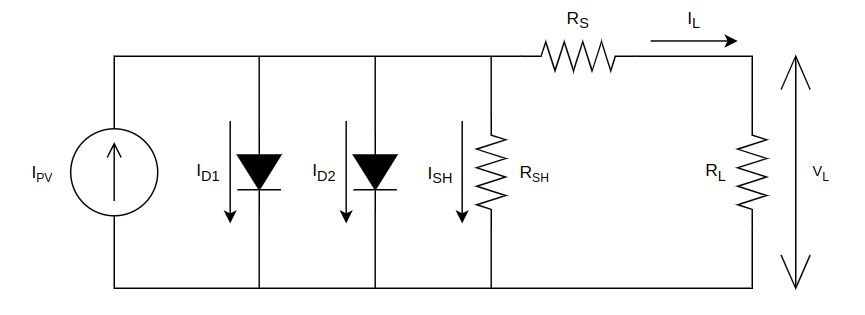
\includegraphics[width=\textwidth]{solar_cell_seven_parameter_model.png}
    \caption{Seven Parameter, or Double Diode Model of a Solar Cell}
    \label{fig:double_diode_model}
\end{figure}

The seven parameter solar cell model (\autoref{fig:double_diode_model}), also
known as a double diode model, builds upon the five parameter model by
introducing a second diode (hence the name) to more accurately model internal
current losses.

These losses can be split into the following:

\begin{itemize}
    \item losses due to carrier recombination in the space charge region of the
    P-N junction,
    \item and losses due to surface recombination.
\end{itemize}

These currents are denoted as \acf{ID1} and \acf{ID2}, respectively. By
differentiating between the two primary recombination processes in the cell, the
seven parameter model is generally considered more accurate than the five
parameter model.

The general form of this equation is shown in \autoref{eq:cell_output_current_7}.

\begin{equation}
    I_L = I_{PV} - I_{D1} - I_{D2} - I_{SH}
    \equnit{\si{\ampere}}
    \label{eq:cell_output_current_7}
\end{equation}

This results in the \autoref{eq:cell_output_current_8} when all components have
been inserted:

\begin{equation}
    \begin{split}
        I_L(V_L, G, T_C) &= I_{PV}(G, T_C, R_S, R_{SH})
                          - I_{D1}(V_L, G, T_C, R_S)
                          - I_{D2}(V_L, G, T_C, R_S) \\
        & \quad           - I_{SH}(R_S, R_{SH}) \\
        &                 = I_{SC}(G, T_C)\frac{R_S + R_{SH}}{R_{SH}}
                          - I_{01}(G, T_C)[\exp(\frac{q[V_L + I_L R_S]}{n_1 k_B T_C}) - 1] \\
        & \quad           - I_{02}(G, T_C)[\exp(\frac{q[V_L + I_L R_S]}{n_2 k_B T_C}) - 1]
                          - \frac{V_L + I_L R_S}{R_{SH}} \\
        &                 = I_{SC}(G, T_C)\frac{R_S + R_{SH}}{R_{SH}}
                          - I_{SC}(G, T_C)\frac{\exp(\frac{q[V_L + I_L R_S]}{n_1 k_B T_C}) - 1}{\exp(\frac{qV_{OC}(G, T_C)}{n_1 k_B T_C}) - 1} \\
        & \quad           - I_{SC}(G, T_C)\frac{\exp(\frac{q[V_L + I_L R_S]}{n_2 k_B T_C}) - 1}{\exp(\frac{qV_{OC}(G, T_C)}{n_2 k_B T_C}) - 1}
                          - \frac{V_L + I_L R_S}{R_{SH}} \\
        &                 = I_{SC}(G, T_C)[
                                \frac{R_S + R_{SH}}{R_{SH}}
                              + \frac{1 - \exp(\frac{q[V_L + I_L R_S]}{n_1 k_B T_C})}{1 - \exp(\frac{qV_{OC}(G, T_C)}{n_1 k_B T_C})} \\
        & \quad               + \frac{1 - \exp(\frac{q[V_L + I_L R_S]}{n_2 k_B T_C})}{1 - \exp(\frac{qV_{OC}(G, T_C)}{n_2 k_B T_C})}]
                          - \frac{V_L + I_L R_S}{R_{SH}}
    \end{split}
    \equnit{\si{\ampere}}
    \label{eq:cell_output_current_8}
\end{equation}

We note in this equation \ac{VT} was substituted back in to demonstrate that
each ideality constant for each diode is unique.

\newpage
\todo[inline]{Behold! True evil!!!\newline Not for general consumption.}
\begin{equation}
    \begin{split}
        I_L(V_L, G, T_C) &= I_{SC,ref}\frac{G}{G_{ref}}[1 - \alpha(T_{C,ref} - T_C)] \\
        & \quad             [ \\
        & \quad\quad            \frac{R_{S,ref} \exp(\zeta [T_{C,ref} - T_C])[1 + \eta(G - G_{ref})]}{R_{SH,ref} \exp(\kappa [T_{C,ref} - T_C])[1 - \iota(G - G_{ref})]} + 1 \\
        & \quad\quad          + \frac{1 - \exp(\frac{q[V_L + I_L R_{S,ref} \exp(\zeta [T_{C,ref} - T_C])[1 + \eta(G - G_{ref})]]}{n_1 k_B T_C})}{1 - \exp(\frac{q[V_{OC,ref}[1 - \beta (T_{C,ref} - T_C)] + \frac{nk_B(T_{C,ref} + T_C/\gamma)}{q}\ln(\frac{G}{G_{ref}})](G, T_C)}{n_1 k_B T_C})} \\
        & \quad\quad          + \frac{1 - \exp(\frac{q[V_L + I_L R_{S,ref} \exp(\zeta [T_{C,ref} - T_C])[1 + \eta(G - G_{ref})]]}{n_2 k_B T_C})}{1 - \exp(\frac{q[V_{OC,ref}[1 - \beta (T_{C,ref} - T_C)] + \frac{nk_B(T_{C,ref} + T_C/\gamma)}{q}\ln(\frac{G}{G_{ref}})](G, T_C)}{n_2 k_B T_C})} \\
        & \quad             ] \\
        & \quad             - \frac{V_L + I_L R_{S,ref} \exp(\zeta [T_{C,ref} - T_C])[1 + \eta(G - G_{ref})]}{R_{SH,ref} \exp(\kappa [T_{C,ref} - T_C])[1 - \iota(G - G_{ref})]}
    \end{split}
    \equnit{\si{\ampere}}
    \label{eq:cell_output_current_9}
\end{equation}

\todo[inline]{See \url{https://www.desmos.com/calculator/69rs9uo14f} to play
around with the complete seven parameter solar cell model. Add as a figure later
on compared to experimental data.}


\subsubsection{Model Summary}\label{subsubsec:seven_param_model_summary}

\todo[inline]{Might want to look for some more novel content, or wrap this section up as
is. Nothing particularly new here besides another parameter to estimate.}


